\documentclass[11pt,a4paper]{article}

\usepackage[margin=2.3cm]{geometry}
\usepackage[T1]{fontenc}
\usepackage[utf8]{inputenc}
\usepackage{lmodern}
\usepackage{microtype}
\usepackage{setspace}
\usepackage{enumitem}
\usepackage{booktabs}
\usepackage{longtable}
\usepackage{array}
\usepackage{tabularx}
\usepackage{xcolor}
\usepackage[hidelinks]{hyperref}
\usepackage{tikz}
\usetikzlibrary{positioning,shapes.geometric,arrows.meta,fit,calc,backgrounds}

\setstretch{1.08}
\setlist[itemize]{leftmargin=1.4em,itemsep=0.25em,topsep=0.35em}
\setlist[enumerate]{leftmargin=1.5em,itemsep=0.25em,topsep=0.35em}

\definecolor{ink}{HTML}{0F172A}
\definecolor{accent}{HTML}{1D4ED8}
\definecolor{soft}{HTML}{EFF6FF}
\definecolor{line}{HTML}{334155}
\definecolor{muted}{HTML}{64748B}
\definecolor{store}{HTML}{ECFDF5}
\definecolor{warn}{HTML}{FFF7ED}

\tikzset{
  svc/.style={draw=line, fill=soft, rounded corners=2pt, align=center,
              font=\scriptsize, inner sep=4pt, minimum height=9mm},
  proc/.style={draw=line, fill=soft, circle, align=center, font=\scriptsize,
               inner sep=1pt, minimum size=16mm},
  store/.style={draw=line, fill=store, align=center, font=\scriptsize,
                inner sep=3pt, minimum height=8mm,
                shape=cylinder, shape border rotate=90, aspect=0.25},
  ext/.style={draw=line, fill=warn, align=center, font=\scriptsize,
              inner sep=3pt, minimum height=8mm},
  uc/.style={draw=line, fill=white, ellipse, align=center, font=\scriptsize,
             inner sep=2pt, minimum width=28mm},
  cls/.style={draw=line, fill=white, align=center, font=\scriptsize,
              inner sep=3pt, minimum width=34mm},
  flow/.style={-{Stealth[length=2.2mm]}, draw=line, font=\tiny},
  dashflow/.style={-{Stealth[length=2.2mm]}, draw=muted, dashed, font=\tiny},
  entity/.style={draw=line, fill=soft, align=center, font=\scriptsize\bfseries,
                 inner sep=4pt, minimum width=28mm, minimum height=7mm},
  rel/.style={draw=line, fill=white, diamond, aspect=2.2, align=center,
              font=\tiny, inner sep=1pt}
}

\title{\textbf{FounderVoice}\\[0.4em]
\large Architecture Document}
\author{FounderVoice}
\date{}

\begin{document}
\maketitle
\thispagestyle{empty}

\begin{abstract}
\noindent
FounderVoice turns a founder's spoken or written account of a company into a structured Claim Graph, an investor critic, and a diligence pack (a slide deck and a workbook). This document specifies that system as a \textbf{microservices} architecture. Each service owns one business capability and its own data. Clients reach the system through an API gateway. The speech-to-export pipeline is coordinated by a message queue, while user edits travel over synchronous HTTP APIs. The database section gives the entity-relationship model, the physical schema owned by each service, and the data-exchange contract: how often data moves, which data sets move, and whether the mode is an API, a file, or a queue.
\end{abstract}

\tableofcontents
\newpage

%---------------------------------------------------------------------
\section{Application}
%---------------------------------------------------------------------

\subsection{Microservices}

FounderVoice is designed as a set of independently deployable services. The product loop is Capture, Structure, Stress-test, Resolve, and Render. Each stage is a bounded context with its own deployable unit, its own database, and a published contract. A failure or a scale-up in speech transcription does not require redeploying claim editing or deck rendering.

The team selected microservices because the workload is uneven. Speech transcription is CPU-heavy and bursty. Claim extraction and the investor critic are model calls with different latency and cost. Deck and workbook rendering is I/O-heavy and runs only when a founder asks for a pack. Identity, projects, and claim edits are ordinary request-response traffic. Splitting these capabilities lets each one scale, fail, and ship on its own release cycle. Shared rules stay in one place: agents draft claims, founders confirm them, numeric assumptions appear only when the founder stated a number, and a strict-mode export stays watermarked until critical questions are answered and claims are confirmed.

\subsubsection{Service catalogue}

\begin{table}[ht]
\centering
\caption{FounderVoice microservices}
\label{tab:services}
\small
\begin{tabularx}{\textwidth}{@{}l X@{}}
\toprule
\textbf{Service} & \textbf{Responsibility} \\
\midrule
API Gateway &
Single public entry for the web app and the mobile app. Verifies the caller, routes HTTP, and composes read models. \\
Identity Service &
Registration, sign-in, and profiles. A profile is a founder or an investor, with display name, organisation, and terms acceptance. \\
Project Service &
Fundraising projects: name, founder, language, strict mode, status, and the published readiness score. \\
Speech Service &
Audio ingest. Denoise, detect Hindi or English, transcribe, and translate non-English speech into an English working transcript. \\
Claim Graph Service &
Ontology and extraction. Typed claims (problem, solution, traction, ask, and the rest of the deck slots), provenance, and founder edits. \\
Critic Service &
Investor questions tied to claim types, with severity, rationale, and founder answers. \\
Audit Service &
Readiness score and issue list: open critical questions, unconfirmed claims, placeholder assumptions, and soft traction. \\
Export Service &
Renders the confirmed graph into a PPTX deck and an XLSX model, applies the watermark when strict mode is not satisfied, and serves downloads. \\
\bottomrule
\end{tabularx}
\end{table}

\subsubsection{How the services collaborate}

Clients never call internal services directly. The web client (Next.js) and the mobile client (React Native with Expo) talk only to the API Gateway over HTTPS.

Two interaction styles are used, and both are part of the microservice design:

\begin{itemize}
  \item \textbf{Synchronous HTTP.} Create a project, edit a claim, answer a question, refresh the audit, and request an export. The gateway calls the owning service and returns JSON.
  \item \textbf{Asynchronous queue.} After a memo is stored, the gateway publishes \texttt{memo.stored}. The Speech Service consumes it and publishes \texttt{transcript.ready}. The Claim Graph Service publishes \texttt{claims.extracted}. The Critic Service and the Audit Service consume that event. The Export Service runs only on \texttt{export.requested}.
\end{itemize}

Each service owns its tables. Another service stores a \texttt{project\_id} or \texttt{memo\_id} as a reference, not as a cross-database foreign key. Files (source audio, pasted text, PPTX, XLSX) live in an object store. The queue carries event notices and identifiers. Payloads that must be durable are written to the owning database or the object store, then referenced by id.

\subsubsection{Claim ontology}

The Claim Graph Service is the source of truth for what a founder has actually said. Claim types, in deck order, are: problem, why now, insight, solution, ideal customer, market, traction, go-to-market, pricing, unit economics, competition, differentiation, team, the ask, use of funds, milestones, and risk. A claim has a status (\texttt{draft}, \texttt{stated}, \texttt{inferred}, \texttt{challenged}, \texttt{confirmed}, \texttt{rejected}) and a provenance (\texttt{founder\_stated}, \texttt{inferred}, \texttt{benchmark}, \texttt{placeholder}, \texttt{verified\_metric}). Extraction may use a local heuristic or an optional language model. In both cases the working transcript is English, and the original-language transcript is kept on the memo.

\subsubsection{Honesty invariant}

The Audit Service enforces the product rule across service boundaries. Critical unanswered questions and unconfirmed claims block a clean export when the project is in strict mode. Placeholder assumptions cannot be presented as founder-stated numbers. The Export Service reads the latest audit snapshot and sets \texttt{watermarked} on every artifact until the audit reports the pack as investor-ready. Downloads still succeed. The watermark is the signal, not a hard lock.

%---------------------------------------------------------------------
\subsection{Use case diagram}
%---------------------------------------------------------------------

\begin{figure}[ht]
\centering
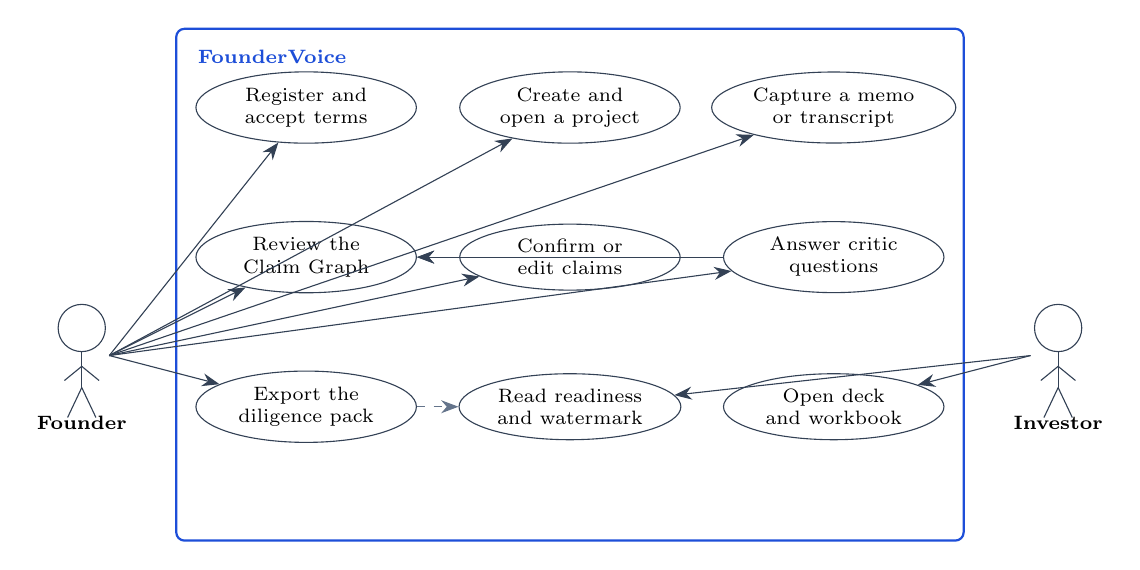
\begin{tikzpicture}[x=1cm,y=1cm]
  \draw[accent, thick, rounded corners=3pt] (1.55,-0.15) rectangle (11.55,6.35);
  \node[font=\scriptsize\bfseries, text=accent, anchor=north west] at (1.7,6.2) {FounderVoice};

  \node[circle, draw=line, minimum size=6mm, inner sep=0pt] (fh) at (0.35,2.55) {};
  \draw[line] (fh.south) -- ++(0,-0.45);
  \draw[line] ($(fh.south)+(0,-0.18)$) -- ++(-0.22,-0.18);
  \draw[line] ($(fh.south)+(0,-0.18)$) -- ++(0.22,-0.18);
  \draw[line] ($(fh.south)+(0,-0.45)$) -- ++(-0.18,-0.38);
  \draw[line] ($(fh.south)+(0,-0.45)$) -- ++(0.18,-0.38);
  \node[font=\scriptsize\bfseries] at (0.35,1.35) {Founder};

  \node[circle, draw=line, minimum size=6mm, inner sep=0pt] (ih) at (12.75,2.55) {};
  \draw[line] (ih.south) -- ++(0,-0.45);
  \draw[line] ($(ih.south)+(0,-0.18)$) -- ++(-0.22,-0.18);
  \draw[line] ($(ih.south)+(0,-0.18)$) -- ++(0.22,-0.18);
  \draw[line] ($(ih.south)+(0,-0.45)$) -- ++(-0.18,-0.38);
  \draw[line] ($(ih.south)+(0,-0.45)$) -- ++(0.18,-0.38);
  \node[font=\scriptsize\bfseries] at (12.75,1.35) {Investor};

  \node[uc] (reg) at (3.2,5.35) {Register and\\accept terms};
  \node[uc] (proj) at (6.55,5.35) {Create and\\open a project};
  \node[uc] (cap) at (9.9,5.35) {Capture a memo\\or transcript};
  \node[uc] (graph) at (3.2,3.45) {Review the\\Claim Graph};
  \node[uc] (confirm) at (6.55,3.45) {Confirm or\\edit claims};
  \node[uc] (answer) at (9.9,3.45) {Answer critic\\questions};
  \node[uc] (export) at (3.2,1.55) {Export the\\diligence pack};
  \node[uc] (read) at (6.55,1.55) {Read readiness\\and watermark};
  \node[uc] (pack) at (9.9,1.55) {Open deck\\and workbook};

  \draw[flow] (0.7,2.2) -- (reg);
  \draw[flow] (0.7,2.2) -- (proj);
  \draw[flow] (0.7,2.2) -- (cap);
  \draw[flow] (0.7,2.2) -- (graph);
  \draw[flow] (0.7,2.2) -- (confirm);
  \draw[flow] (0.7,2.2) -- (answer);
  \draw[flow] (0.7,2.2) -- (export);
  \draw[flow] (12.4,2.2) -- (read);
  \draw[flow] (12.4,2.2) -- (pack);
  \draw[flow] (confirm) -- (graph);
  \draw[flow] (answer) -- (graph);
  \draw[dashflow] (export) -- (read);
\end{tikzpicture}
\caption{Use cases. The founder owns capture, confirmation, and export. The investor reads readiness and the rendered pack.}
\label{fig:usecase}
\end{figure}

The founder registers, accepts terms, and creates a project. Capture accepts a live recording, an uploaded audio file, or a pasted transcript. The Claim Graph and the critic questions are drafts until the founder confirms claims and writes answers. Export always produces files. The investor's use cases are read-only: readiness, the watermark state, and the deck and workbook.

%---------------------------------------------------------------------
\subsection{Class diagram}
%---------------------------------------------------------------------

\begin{figure}[ht]
\centering
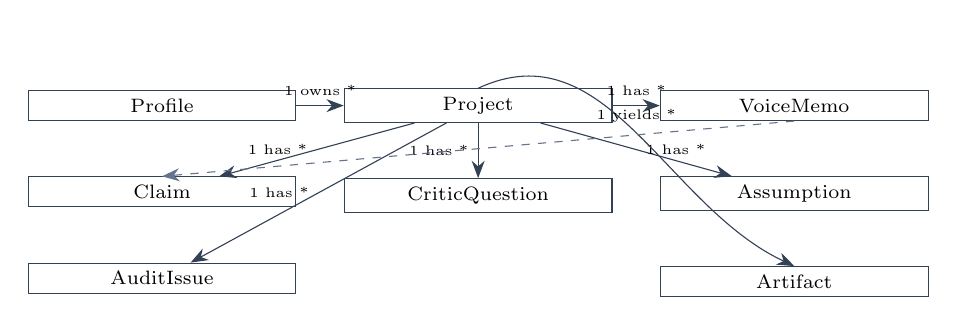
\begin{tikzpicture}[node distance=7mm and 6mm]
  \node[cls] (profile) {Profile};
  \node[cls, right=of profile] (project) {Project};
  \node[cls, right=of project] (memo) {VoiceMemo};
  \node[cls, below=of profile] (claim) {Claim};
  \node[cls, below=of project] (question) {CriticQuestion};
  \node[cls, below=of memo] (assumption) {Assumption};
  \node[cls, below=of claim] (issue) {AuditIssue};
  \node[cls, below=of assumption] (artifact) {Artifact};

  \draw[flow] (profile) -- node[above, font=\tiny] {1 owns *} (project);
  \draw[flow] (project) -- node[above, font=\tiny] {1 has *} (memo);
  \draw[flow] (project) -- node[left, font=\tiny] {1 has *} (claim);
  \draw[flow] (project) -- node[left, font=\tiny] {1 has *} (question);
  \draw[flow] (project) -- node[right, font=\tiny] {1 has *} (assumption);
  \draw[flow] (project) -- node[left, font=\tiny] {1 has *} (issue);
  \draw[flow] (project.north) to[out=25,in=155] node[above, font=\tiny] {1 yields *} (artifact.north);
  \draw[dashflow] (memo.south) -- (claim.north);
\end{tikzpicture}
\caption{Domain classes. Dashed link: a claim cites the memo it was extracted from. Persistence of each class is owned by the microservice named in the schema section.}
\label{fig:class}
\end{figure}

\begin{table}[ht]
\centering
\caption{Principal attributes}
\label{tab:classattrs}
\small
\begin{tabularx}{\textwidth}{@{}l X@{}}
\toprule
\textbf{Class} & \textbf{Attributes} \\
\midrule
Profile & id, role (founder $\mid$ investor), display name, organisation, email, terms accepted, auth provider \\
Project & id, name, founder name, language, output language, strict mode, status, readiness score, summary \\
VoiceMemo & id, project id, filename, stored path, content type, language, English transcript, original transcript, duration, status \\
Claim & id, project id, claim type, title, body, status, confidence, provenance, numeric value, unit, source quote, source memo id \\
CriticQuestion & id, project id, claim type, severity, question, rationale, answer, resolved \\
Assumption & id, project id, key, label, value, unit, provenance, notes \\
AuditIssue & id, project id, code, severity, message, related claim ids, resolved \\
Artifact & id, project id, kind (pptx $\mid$ xlsx), filename, stored path, watermarked, metadata \\
\bottomrule
\end{tabularx}
\end{table}

%---------------------------------------------------------------------
\subsection{Data-flow diagram}
%---------------------------------------------------------------------

\subsubsection{Context diagram (Level 0)}

\begin{figure}[ht]
\centering
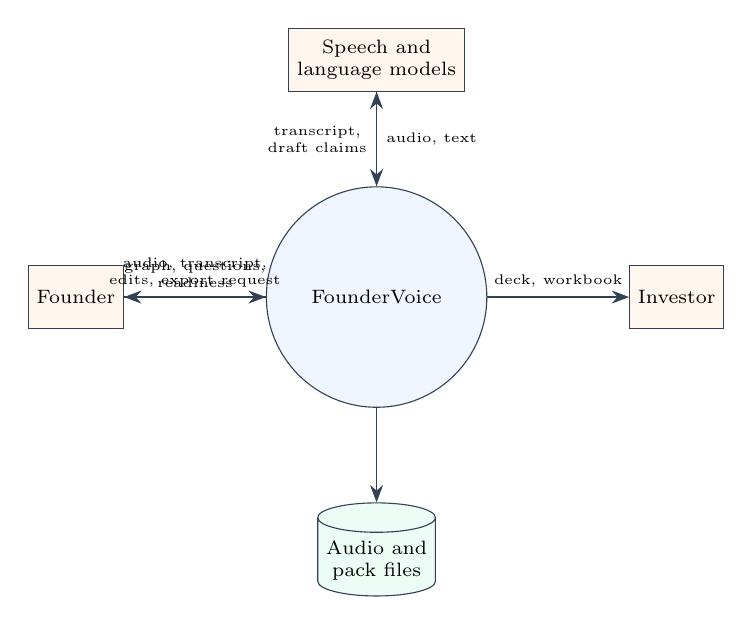
\begin{tikzpicture}[node distance=11mm]
  \node[ext] (founder) {Founder};
  \node[proc, right=18mm of founder, minimum size=28mm] (sys) {FounderVoice};
  \node[ext, right=18mm of sys] (investor) {Investor};
  \node[ext, above=12mm of sys] (model) {Speech and\\language models};
  \node[store, below=12mm of sys] (files) {Audio and\\pack files};

  \draw[flow] (founder) -- node[above, font=\tiny, align=center] {audio, transcript,\\edits, export request} (sys);
  \draw[flow] (sys) -- node[above, font=\tiny, align=center] {graph, questions,\\readiness} (founder);
  \draw[flow] (sys) -- node[above, font=\tiny] {deck, workbook} (investor);
  \draw[flow] (sys) -- node[right, font=\tiny] {audio, text} (model);
  \draw[flow] (model) -- node[left, font=\tiny, align=center] {transcript,\\draft claims} (sys);
  \draw[flow] (sys) -- (files);
\end{tikzpicture}
\caption{Level 0. FounderVoice is one system to its users. Models and the file store are outside the process boundary.}
\label{fig:dfd0}
\end{figure}

\subsubsection{Level 1}

\begin{figure}[ht]
\centering
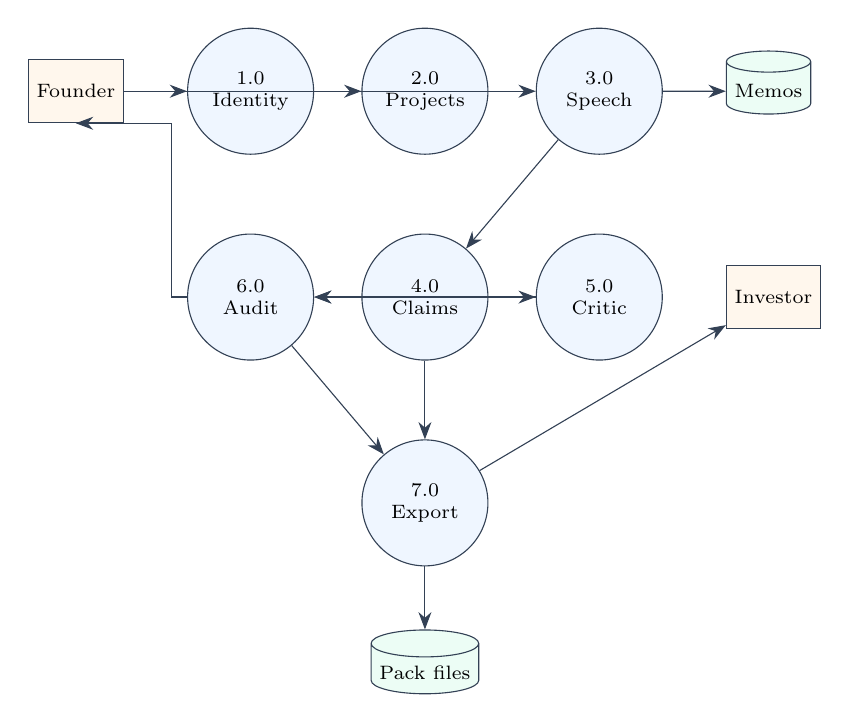
\begin{tikzpicture}[node distance=4mm and 3mm, every node/.style={font=\scriptsize}]
  \node[ext] (f) {Founder};
  \node[proc, right=8mm of f] (p1) {1.0\\Identity};
  \node[proc, right=6mm of p1] (p2) {2.0\\Projects};
  \node[proc, right=6mm of p2] (p3) {3.0\\Speech};
  \node[proc, below=10mm of p2] (p4) {4.0\\Claims};
  \node[proc, right=6mm of p4] (p5) {5.0\\Critic};
  \node[proc, left=6mm of p4] (p6) {6.0\\Audit};
  \node[proc, below=10mm of p4] (p7) {7.0\\Export};
  \node[store, right=8mm of p3] (dspeech) {Memos};
  \node[store, below=8mm of p7] (dfiles) {Pack files};
  \node[ext, right=8mm of p5] (inv) {Investor};

  \draw[flow] (f) -- (p1);
  \draw[flow] (f.east) -- ++(0.15,0) |- (p2);
  \draw[flow] (f.east) -- ++(0.3,0) |- (p3);
  \draw[flow] (p3) -- (dspeech);
  \draw[flow] (p3) -- (p4);
  \draw[flow] (p4) -- (p5);
  \draw[flow] (p4) -- (p6);
  \draw[flow] (p5) -- (p6);
  \draw[flow] (p6) -- (p7);
  \draw[flow] (p4) -- (p7);
  \draw[flow] (p7) -- (dfiles);
  \draw[flow] (p7) -- (inv);
  \draw[flow] (p6.west) -- ++(-0.2,0) |- (f.south);
\end{tikzpicture}
\caption{Level 1. Numbered processes match the microservices. Speech writes memos. Claims, critic, and audit feed export. Export writes the pack files the investor opens.}
\label{fig:dfd1}
\end{figure}

Data stores in the Level 1 diagram are logical. Physically, memos belong to the Speech Service database plus the object store, and pack files belong to the Export Service plus the object store. Claim, question, assumption, and audit rows sit in the database of the service that creates them.

%---------------------------------------------------------------------
\subsection{Component diagram}
%---------------------------------------------------------------------

\begin{figure}[ht]
\centering
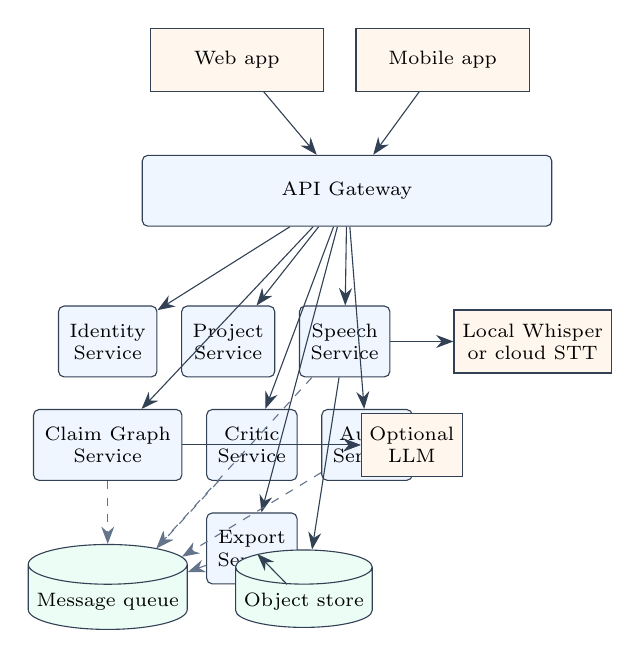
\begin{tikzpicture}[node distance=5mm and 4mm]
  \node[ext, minimum width=22mm] (web) {Web app};
  \node[ext, right=4mm of web, minimum width=22mm] (mobile) {Mobile app};
  \node[svc, below=8mm of web, minimum width=52mm, xshift=14mm] (gw) {API Gateway};

  \node[svc, below left=10mm and -2mm of gw] (id) {Identity\\Service};
  \node[svc, right=3mm of id] (proj) {Project\\Service};
  \node[svc, right=3mm of proj] (speech) {Speech\\Service};
  \node[svc, below=4mm of id] (claims) {Claim Graph\\Service};
  \node[svc, right=3mm of claims] (critic) {Critic\\Service};
  \node[svc, right=3mm of critic] (audit) {Audit\\Service};
  \node[svc, below=4mm of critic] (export) {Export\\Service};

  \node[store, below=8mm of claims] (bus) {Message queue};
  \node[store, right=6mm of bus] (obj) {Object store};
  \node[ext, right=8mm of speech] (whisper) {Local Whisper\\or cloud STT};
  \node[ext, right=8mm of critic] (llm) {Optional\\LLM};

  \draw[flow] (web) -- (gw);
  \draw[flow] (mobile) -- (gw);
  \draw[flow] (gw) -- (id);
  \draw[flow] (gw) -- (proj);
  \draw[flow] (gw) -- (speech);
  \draw[flow] (gw) -- (claims);
  \draw[flow] (gw) -- (critic);
  \draw[flow] (gw) -- (audit);
  \draw[flow] (gw) -- (export);
  \draw[dashflow] (speech) -- (bus);
  \draw[dashflow] (claims) -- (bus);
  \draw[dashflow] (critic) -- (bus);
  \draw[dashflow] (audit) -- (bus);
  \draw[dashflow] (export) -- (bus);
  \draw[flow] (speech) -- (whisper);
  \draw[flow] (claims) -- (llm);
  \draw[flow] (critic) -- (llm);
  \draw[flow] (speech) -- (obj);
  \draw[flow] (export) -- (obj);
\end{tikzpicture}
\caption{Components. Solid arrows are synchronous calls. Dashed arrows are queue publish and consume. Speech and Export also read and write the object store.}
\label{fig:component}
\end{figure}

The API Gateway is a thin component. It authenticates the caller with the Identity Service, then forwards the command to the service that owns the resource. It does not store projects, transcripts, or claims. Model adapters sit behind Speech, Claim Graph, and Critic so a local Whisper model and an optional hosted model are replaceable without changing the other services.

%---------------------------------------------------------------------
\subsection{Sequence diagram}
%---------------------------------------------------------------------

\begin{figure}[ht]
\centering
\begin{tikzpicture}[x=1mm,y=1mm]
  \foreach \x/\name in {0/Founder, 28/Gateway, 52/Speech, 76/Claims, 100/Critic, 124/Audit, 148/Export} {
    \node[font=\scriptsize\bfseries, anchor=south] at (\x,0) {\name};
    \draw[muted] (\x, -2) -- (\x, -118);
  }
  \draw[flow] (0,-8) -- node[above, font=\tiny, sloped] {POST memo (audio)} (28,-8);
  \draw[flow] (28,-16) -- node[above, font=\tiny, sloped] {store file, enqueue} (52,-16);
  \draw[flow] (52,-28) -- node[above, font=\tiny, sloped] {transcript.ready} (76,-28);
  \draw[flow] (76,-40) -- node[above, font=\tiny, sloped] {claims.extracted} (100,-40);
  \draw[flow] (76,-48) -- node[above, font=\tiny, sloped] {claims.extracted} (124,-48);
  \draw[flow] (100,-58) -- node[above, font=\tiny, sloped] {questions.ready} (124,-58);
  \draw[flow] (124,-68) -- node[above, font=\tiny] {readiness} (28,-68);
  \draw[flow] (28,-76) -- node[above, font=\tiny] {graph + questions} (0,-76);

  \draw[flow] (0,-88) -- node[above, font=\tiny, sloped] {confirm claims, answer} (28,-88);
  \draw[flow] (28,-96) -- node[above, font=\tiny] {PATCH claim / answer} (76,-96);
  \draw[flow] (76,-104) -- node[above, font=\tiny] {re-audit} (124,-104);
  \draw[flow] (0,-112) -- node[above, font=\tiny, sloped] {export} (28,-112);
  \node[font=\tiny, anchor=west] at (30,-116) {Gateway then calls Export; Export reads audit and writes PPTX + XLSX.};
\end{tikzpicture}
\caption{Sequence for one memo, founder confirmation, and export. Transcription, extraction, critic, and audit proceed on the queue. Confirmation and export are request-response.}
\label{fig:sequence}
\end{figure}

A pasted transcript skips denoising and speech-to-text. The Speech Service still records a memo with status \texttt{transcribed} and publishes \texttt{transcript.ready}, so Claims, Critic, and Audit stay on the same path. Re-extraction publishes a new \texttt{claims.extracted} and replaces the draft graph for that project version.

%---------------------------------------------------------------------
\subsection{Deployment diagram}
%---------------------------------------------------------------------

\begin{figure}[ht]
\centering
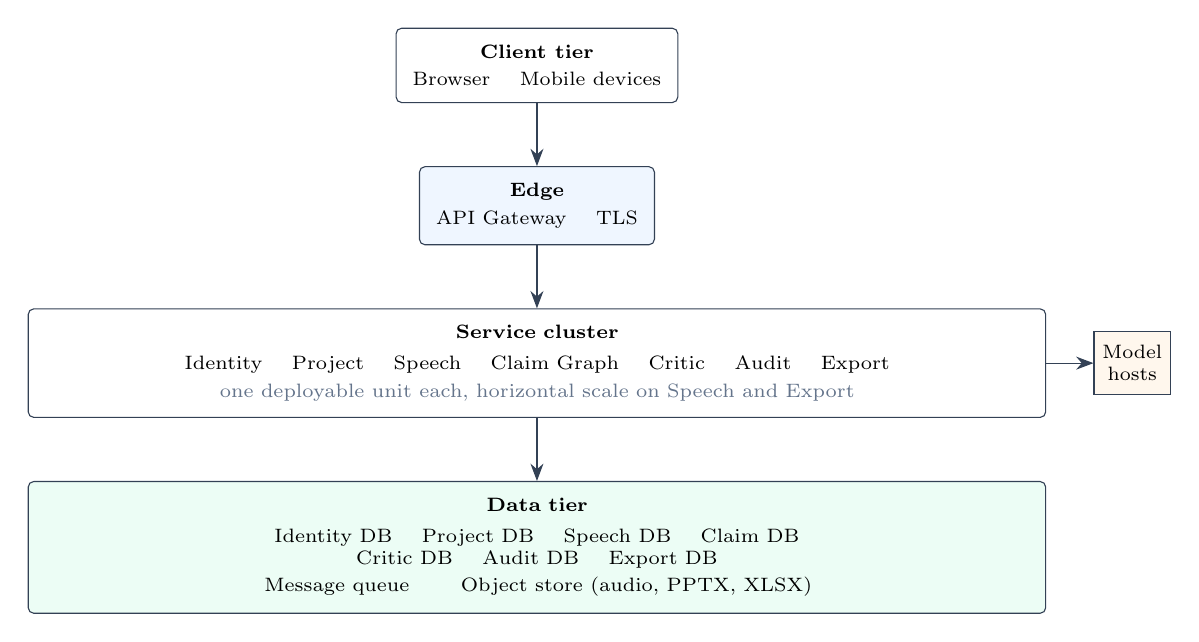
\begin{tikzpicture}[node distance=6mm and 8mm]
  \node[draw=line, rounded corners=2pt, inner sep=6pt, fill=white, align=center, font=\scriptsize] (clients) {
    \textbf{Client tier}\\[2pt]
    Browser \quad Mobile devices
  };
  \node[draw=line, rounded corners=2pt, inner sep=6pt, fill=soft, align=center, font=\scriptsize, below=8mm of clients] (edge) {
    \textbf{Edge}\\[2pt]
    API Gateway \quad TLS
  };
  \node[draw=line, rounded corners=2pt, inner sep=6pt, fill=white, align=center, font=\scriptsize, below=8mm of edge, text width=12.5cm] (cluster) {
    \textbf{Service cluster}\\[3pt]
    Identity \quad Project \quad Speech \quad Claim Graph \quad Critic \quad Audit \quad Export\\[2pt]
    {\color{muted} one deployable unit each, horizontal scale on Speech and Export}
  };
  \node[draw=line, rounded corners=2pt, inner sep=6pt, fill=store, align=center, font=\scriptsize, below=8mm of cluster, text width=12.5cm] (data) {
    \textbf{Data tier}\\[3pt]
    Identity DB \quad Project DB \quad Speech DB \quad Claim DB\\
    Critic DB \quad Audit DB \quad Export DB\\[2pt]
    Message queue \qquad Object store (audio, PPTX, XLSX)
  };
  \node[ext, right=6mm of cluster] (models) {Model\\hosts};

  \draw[flow] (clients) -- (edge);
  \draw[flow] (edge) -- (cluster);
  \draw[flow] (cluster) -- (data);
  \draw[flow] (cluster) -- (models);
\end{tikzpicture}
\caption{Deployment. Clients stop at the gateway. Each microservice runs as its own unit and connects only to its database, the queue, and, where needed, the object store or a model host.}
\label{fig:deploy}
\end{figure}

Speech is deployed with access to a local Whisper runtime by default, so transcription does not depend on an external key. A configuration switch sends the same audio contract to a hosted speech API. Claim Graph and Critic call a language model only when that option is enabled. Otherwise they run the in-process heuristic and still emit the same events. The object store is private. Download URLs are issued by the Export Service after it checks the caller's project access with the Project Service.

%---------------------------------------------------------------------
\section{Database}
%---------------------------------------------------------------------

Microservices do not share one database. The diagram below is the logical model of FounderVoice. The schema section then assigns each table to the service that owns it. Cross-service links are identifier references.

\subsection{ER diagram}

\begin{figure}[ht]
\centering
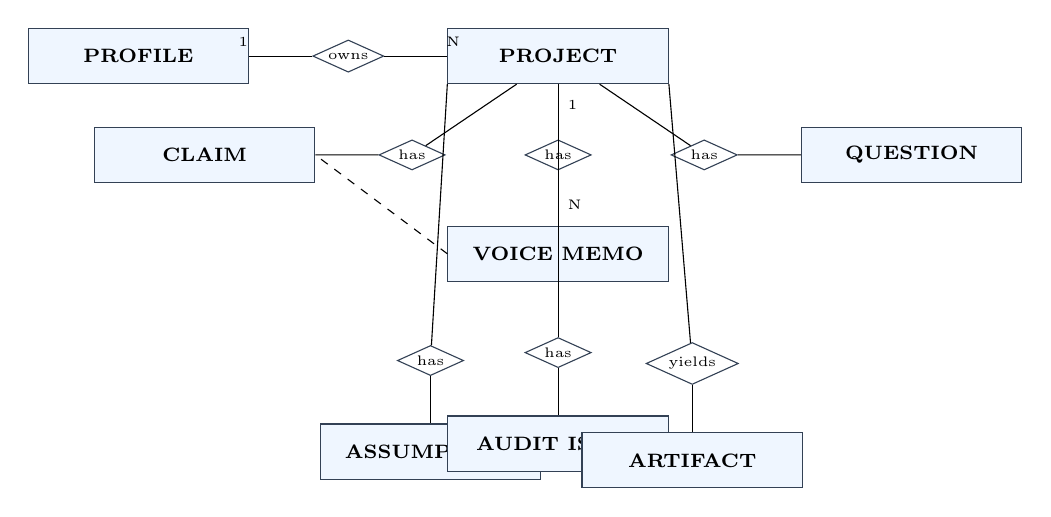
\begin{tikzpicture}[node distance=5mm and 7mm]
  \node[entity] (profile) {PROFILE};
  \node[rel, right=8mm of profile] (owns) {owns};
  \node[entity, right=8mm of owns] (project) {PROJECT};

  \node[rel, below=7mm of project] (hasm) {has};
  \node[entity, below=7mm of hasm] (memo) {VOICE MEMO};

  \node[rel, left=10mm of hasm] (hasc) {has};
  \node[entity, left=8mm of hasc] (claim) {CLAIM};

  \node[rel, right=10mm of hasm] (hasq) {has};
  \node[entity, right=8mm of hasq] (question) {QUESTION};

  \node[rel, below left=9mm and 0mm of memo] (hasa) {has};
  \node[entity, below=6mm of hasa] (assumption) {ASSUMPTION};

  \node[rel, below=7mm of memo] (hasu) {has};
  \node[entity, below=6mm of hasu] (issue) {AUDIT ISSUE};

  \node[rel, below right=9mm and 0mm of memo] (hasf) {yields};
  \node[entity, below=6mm of hasf] (artifact) {ARTIFACT};

  \draw (profile) -- (owns) -- (project);
  \draw (project) -- (hasm) -- (memo);
  \draw (project) -- (hasc) -- (claim);
  \draw (project) -- (hasq) -- (question);
  \draw (project.south west) -- (hasa);
  \draw (hasa) -- (assumption);
  \draw (project.south) -- (hasu) -- (issue);
  \draw (project.south east) -- (hasf);
  \draw (hasf) -- (artifact);
  \draw[dashed] (memo.west) -- (claim.east);

  \node[font=\tiny, above] at ($(profile)!0.5!(owns)$) {1};
  \node[font=\tiny, above] at ($(owns)!0.5!(project)$) {N};
  \node[font=\tiny, right] at ($(project)!0.5!(hasm)$) {1};
  \node[font=\tiny, right] at ($(hasm)!0.5!(memo)$) {N};
\end{tikzpicture}
\caption{Logical ER diagram. Cardinality from project outward is one-to-many for memos, claims, questions, assumptions, audit issues, and artifacts. A memo is the provenance source for the claims extracted from it.}
\label{fig:er}
\end{figure}

\begin{table}[ht]
\centering
\caption{Relationship summary}
\label{tab:rels}
\small
\begin{tabular}{@{}llll@{}}
\toprule
\textbf{From} & \textbf{To} & \textbf{Cardinality} & \textbf{Rule} \\
\midrule
Profile & Project & 1:N & A founder owns many projects. Investors do not create projects. \\
Project & Voice memo & 1:N & Every capture, upload, or paste is a memo. \\
Project & Claim & 1:N & One current graph per project; re-extract replaces drafts. \\
Project & Critic question & 1:N & Questions are regenerated with the graph. \\
Project & Assumption & 1:N & A row exists only when a number was stated or marked placeholder. \\
Project & Audit issue & 1:N & Replaced on each audit run. \\
Project & Artifact & 1:N & Each export adds a deck and a workbook. \\
Voice memo & Claim & 1:N & \texttt{source\_memo\_id} on the claim. \\
\bottomrule
\end{tabular}
\end{table}

\subsection{Schema design}

Identifiers are UUID strings. Timestamps are stored in UTC. Boolean flags default as shown. Text fields are unbounded except where a length is given. Each subsection is the schema of one service database.

\subsubsection{Identity Service --- \texttt{identity\_db}}

\begin{table}[ht]
\centering
\caption{\texttt{profiles}}
\small
\begin{tabular}{@{}llll@{}}
\toprule
\textbf{Column} & \textbf{Type} & \textbf{Null} & \textbf{Notes} \\
\midrule
id & uuid & no & Primary key. Same id as the auth user. \\
role & text & no & \texttt{founder} or \texttt{investor}. \\
display\_name & text & no & Default empty string. \\
org\_name & text & no & Default empty string. \\
email & text & no & Default empty string. \\
terms\_accepted & boolean & no & Default false. \\
auth\_provider & text & no & Default \texttt{email}. \\
created\_at & timestamptz & no & \\
updated\_at & timestamptz & no & \\
\bottomrule
\end{tabular}
\end{table}

Row access is limited to the signed-in user. A new auth user inserts one profile. Role, display name, organisation, and terms acceptance are taken from sign-up metadata.

\subsubsection{Project Service --- \texttt{project\_db}}

\begin{table}[ht]
\centering
\caption{\texttt{projects}}
\small
\begin{tabular}{@{}llll@{}}
\toprule
\textbf{Column} & \textbf{Type} & \textbf{Null} & \textbf{Notes} \\
\midrule
id & varchar(36) & no & Primary key. \\
owner\_id & uuid & no & Reference to \texttt{profiles.id}. \\
name & varchar(200) & no & \\
founder\_name & varchar(200) & no & Default empty. \\
language & varchar(16) & no & Default \texttt{en}. Capture language. \\
output\_language & varchar(16) & no & Default \texttt{en}. \\
strict\_mode & boolean & no & Default true. \\
status & varchar(40) & no & Default \texttt{draft}. \\
readiness\_score & float & no & Default 0. Written from audit events. \\
summary & text & no & Default empty. Written from extraction. \\
created\_at & timestamptz & no & \\
updated\_at & timestamptz & no & \\
\bottomrule
\end{tabular}
\end{table}

\subsubsection{Speech Service --- \texttt{speech\_db}}

\begin{table}[ht]
\centering
\caption{\texttt{voice\_memos}}
\small
\begin{tabular}{@{}llll@{}}
\toprule
\textbf{Column} & \textbf{Type} & \textbf{Null} & \textbf{Notes} \\
\midrule
id & varchar(36) & no & Primary key. \\
project\_id & varchar(36) & no & Reference to \texttt{projects.id}. Indexed. \\
filename & varchar(255) & no & \\
stored\_path & varchar(500) & no & Object-store key. \\
content\_type & varchar(100) & no & Audio MIME type or \texttt{text/plain}. \\
language & varchar(16) & no & Detected source language. \\
transcript & text & no & English working copy. \\
original\_transcript & text & no & Source-language text. \\
duration\_seconds & float & no & Default 0. \\
status & varchar(40) & no & \texttt{uploaded}, \texttt{transcribed}, \texttt{translated}, \texttt{stt\_unavailable}. \\
created\_at & timestamptz & no & \\
\bottomrule
\end{tabular}
\end{table}

\subsubsection{Claim Graph Service --- \texttt{claim\_db}}

\begin{table}[ht]
\centering
\caption{\texttt{claim\_nodes}}
\small
\begin{tabular}{@{}llll@{}}
\toprule
\textbf{Column} & \textbf{Type} & \textbf{Null} & \textbf{Notes} \\
\midrule
id & varchar(36) & no & Primary key. \\
project\_id & varchar(36) & no & Indexed. \\
claim\_type & varchar(64) & no & Ontology value, for example \texttt{traction}. \\
title & varchar(300) & no & \\
body & text & no & \\
status & varchar(32) & no & Default \texttt{draft}. \\
confidence & float & no & 0 to 1. Default 0.5. \\
provenance & varchar(40) & no & Default \texttt{founder\_stated}. \\
numeric\_value & float & yes & \\
numeric\_unit & varchar(40) & yes & \\
source\_quote & text & yes & Span from the transcript. \\
source\_memo\_id & varchar(36) & yes & Reference to \texttt{voice\_memos.id}. \\
created\_at & timestamptz & no & \\
updated\_at & timestamptz & no & \\
\bottomrule
\end{tabular}
\end{table}

\begin{table}[ht]
\centering
\caption{\texttt{assumptions}}
\small
\begin{tabular}{@{}llll@{}}
\toprule
\textbf{Column} & \textbf{Type} & \textbf{Null} & \textbf{Notes} \\
\midrule
id & varchar(36) & no & Primary key. \\
project\_id & varchar(36) & no & Indexed. \\
key & varchar(80) & no & Stable key used by the workbook. \\
label & varchar(200) & no & \\
value & float & no & Default 0. \\
unit & varchar(40) & no & \\
provenance & varchar(40) & no & Default \texttt{placeholder}. \\
notes & text & no & \\
\bottomrule
\end{tabular}
\end{table}

\subsubsection{Critic Service --- \texttt{critic\_db}}

\begin{table}[ht]
\centering
\caption{\texttt{critic\_questions}}
\small
\begin{tabular}{@{}llll@{}}
\toprule
\textbf{Column} & \textbf{Type} & \textbf{Null} & \textbf{Notes} \\
\midrule
id & varchar(36) & no & Primary key. \\
project\_id & varchar(36) & no & Indexed. \\
claim\_type & varchar(64) & yes & Null when the question spans the graph. \\
severity & varchar(20) & no & Default \texttt{medium}. Includes \texttt{critical}. \\
question & text & no & \\
rationale & text & no & \\
answer & text & no & Founder reply. Default empty. \\
resolved & boolean & no & True when the answer is non-empty. \\
created\_at & timestamptz & no & \\
\bottomrule
\end{tabular}
\end{table}

\subsubsection{Audit Service --- \texttt{audit\_db}}

\begin{table}[ht]
\centering
\caption{\texttt{audit\_issues}}
\small
\begin{tabular}{@{}llll@{}}
\toprule
\textbf{Column} & \textbf{Type} & \textbf{Null} & \textbf{Notes} \\
\midrule
id & varchar(36) & no & Primary key. \\
project\_id & varchar(36) & no & Indexed. \\
code & varchar(80) & no & For example \texttt{unconfirmed\_claims}. \\
severity & varchar(20) & no & \texttt{block} or \texttt{warn}. \\
message & text & no & \\
claim\_ids\_csv & varchar(500) & no & Related claim ids. \\
resolved & boolean & no & Default false. \\
\bottomrule
\end{tabular}
\end{table}

The readiness score is not duplicated as a second source of truth inside the Audit Service beyond the run that produced it. The score is published on \texttt{audit.completed} and stored on \texttt{projects.readiness\_score} so project lists can render it without a join across databases.

\subsubsection{Export Service --- \texttt{export\_db}}

\begin{table}[ht]
\centering
\caption{\texttt{artifacts}}
\small
\begin{tabular}{@{}llll@{}}
\toprule
\textbf{Column} & \textbf{Type} & \textbf{Null} & \textbf{Notes} \\
\midrule
id & varchar(36) & no & Primary key. \\
project\_id & varchar(36) & no & Indexed. \\
kind & varchar(40) & no & \texttt{pptx} or \texttt{xlsx}. \\
filename & varchar(255) & no & \\
stored\_path & varchar(500) & no & Object-store key. \\
watermarked & boolean & no & True while strict mode is unsatisfied. \\
meta\_json & text & no & Outline and score snapshot. Default \texttt{\{\}}. \\
created\_at & timestamptz & no & \\
\bottomrule
\end{tabular}
\end{table}

\subsection{Data exchange contract}

Services exchange data only through the contracts in this section. A service does not read another service's tables.

\subsubsection{Frequency of data exchanges}

\begin{table}[ht]
\centering
\caption{When data moves}
\label{tab:freq}
\small
\begin{tabularx}{\textwidth}{@{}l l X@{}}
\toprule
\textbf{Exchange} & \textbf{Frequency} & \textbf{Trigger} \\
\midrule
Session and profile &
On sign-in and on app open &
Founder or investor authenticates. \\
Project create, list, update &
On demand &
Each user action. A founder typically creates a project once per company narrative. \\
Audio or text upload &
Once per capture &
Record, file upload, or pasted transcript. \\
\texttt{memo.stored} &
Once per capture &
Immediately after the object store write succeeds. \\
\texttt{transcript.ready} &
Once per memo &
After denoise, detection, transcription, and translation. Retried if speech fails. \\
\texttt{claims.extracted} &
Once per graph version &
First extract and every re-extract. \\
\texttt{questions.ready} &
Once per graph version &
After the critic finishes for that version. \\
Claim, answer, and assumption edits &
On demand &
Each founder save. Often a burst during review. \\
\texttt{audit.completed} &
Once per mutation &
After extraction and after every edit that can change readiness. \\
\texttt{export.requested} and artifact download &
On demand &
Founder asks for a pack, then downloads each file. \\
\bottomrule
\end{tabularx}
\end{table}

There is no scheduled batch exchange. Cadence follows the founder. A single working session is usually one to a few memos, one extraction, many small edits, and one export.

\subsubsection{Data sets}

\begin{table}[ht]
\centering
\caption{Data sets that cross a service boundary}
\label{tab:datasets}
\small
\begin{tabularx}{\textwidth}{@{}l l X@{}}
\toprule
\textbf{Data set} & \textbf{Producer} & \textbf{Contents} \\
\midrule
Profile &
Identity &
User id, role, display name, organisation, terms accepted. \\
Project record &
Project &
Project id, owner id, name, languages, strict mode, status, readiness score, summary. \\
Memo notice &
Speech &
Memo id, project id, object key, content type, language, status. Transcript text is stored in \texttt{speech\_db} and fetched by id. \\
Transcript body &
Speech &
English transcript, original transcript, detected language, duration. \\
Claim set &
Claim Graph &
Claim id, type, title, body, status, confidence, provenance, numeric value and unit, source quote, source memo id. \\
Assumption set &
Claim Graph &
Key, label, value, unit, provenance, notes. \\
Question set &
Critic &
Question id, claim type, severity, text, rationale, answer, resolved. \\
Audit snapshot &
Audit &
Readiness score and issue rows (code, severity, message, claim ids). \\
Artifact notice &
Export &
Artifact id, kind, filename, object key, watermarked flag. \\
Pack bytes &
Export &
PPTX presentation and XLSX workbook. \\
\bottomrule
\end{tabularx}
\end{table}

Event notices stay small: event name, project id, and the id of the new record. The consumer calls the producer's read API for the full data set. That keeps queue messages stable when a claim body or a transcript grows.

\subsubsection{Mode of exchanges}

\begin{table}[ht]
\centering
\caption{Mode of each exchange}
\label{tab:modes}
\small
\begin{tabularx}{\textwidth}{@{}l l X@{}}
\toprule
\textbf{Path} & \textbf{Mode} & \textbf{Contract} \\
\midrule
Clients to gateway &
API &
HTTPS, JSON. Audio upload is multipart form data. \\
Gateway to services &
API &
HTTP JSON inside the cluster. Resource paths are scoped by project id. \\
Pipeline stages &
Queue &
Durable topic. Events: \texttt{memo.stored}, \texttt{transcript.ready}, \texttt{claims.extracted}, \texttt{questions.ready}, \texttt{audit.completed}, \texttt{export.requested}. At-least-once delivery. Consumers are idempotent on project id plus source record id. \\
Audio, pasted text, PPTX, XLSX &
File &
Object store. Database rows store the key, not the bytes. Download is an authenticated file response from Export. \\
Speech and language models &
API &
Speech sends audio or text. Models return text. The heuristic path makes no external call and still returns the same internal data set. \\
\bottomrule
\end{tabularx}
\end{table}

Representative gateway routes, all under the \texttt{/api} prefix:

\begin{itemize}
  \item \texttt{POST /projects}, \texttt{GET /projects}, \texttt{GET /projects/\{id\}}, \texttt{PATCH /projects/\{id\}}
  \item \texttt{POST /projects/\{id\}/memos} (file) and \texttt{POST /projects/\{id\}/memos/text}
  \item \texttt{PATCH /projects/\{id\}/memos/\{memoId\}} and \texttt{POST .../reextract}
  \item \texttt{PATCH /projects/\{id\}/claims/\{claimId\}} and \texttt{POST .../claims/bulk-status}
  \item \texttt{POST /projects/\{id\}/questions/\{questionId\}/answer}
  \item \texttt{PATCH /projects/\{id\}/assumptions/\{assumptionId\}}
  \item \texttt{POST /projects/\{id\}/audit/refresh}
  \item \texttt{POST /projects/\{id\}/export} and \texttt{GET /artifacts/\{artifactId\}/download}
\end{itemize}

The gateway translates each route into a call on the owning service. File routes stream bytes to the object store and publish a queue event. They do not run transcription inside the gateway process.

\end{document}
